%\documentclass[preprint,tightenlines,showpacs,showkeys,floatfix,
%nofootinbib,superscriptaddress,fleqn]{revtex4} 
\documentclass[floatfix,nofootinbib,superscriptaddress,fleqn]{revtex4-2} 
%\documentclass[aps,epsfig,tightlines,fleqn]{revtex4}
\usepackage[utf]{kotex}
\usepackage[HWP]{dhucs-interword}
\usepackage[dvips]{color}
\usepackage{graphicx}
\usepackage{bm}
%\usepackage{fancyhdr}
%\usepackage{dcolumn}
\usepackage{defcolor}
\usepackage{amsmath}
\usepackage{amsfonts}
\usepackage{amssymb}
\usepackage{amscd}
\usepackage{amsthm}
\usepackage[utf8]{inputenc}
 \usepackage{setspace}
 \usepackage{tikz}
%\pagestyle{fancy}

\begin{document}

\title{\Large 2022년 1학기 물리학 I: Quiz 8}
\author{김현철\footnote{Office: 5S-436D (면담시간 매주
    화요일-16:00$\sim$20:00)}} 
\email{hchkim@inha.ac.kr}
\author{Lee Hui-Jae} 
\email{hjlee6674@inha.edu}

\affiliation{Hadron Theory Group, Department of Physics,
Inha University, Incheon 22212, Republic of Korea }
\date{Spring semester, 2022}

\maketitle

\noindent {\bf 문제 1 [20pt]}
가득 찬 화물용 승강기가 천천히 움직이고
있다. 이 승강기의 질량은 $1\,200$ kg이다. 정지상태에서 출발하여 3.0분
동안 54 m를 올라가서 정지하였다. 승강이 대응추의 질량이 950 kg밖에
되지 않으므로 모터의 도움이 필요하다. 케이블을 통해 모터에 작용하는
평균 일률은 얼마인가?

\noindent {\bf 풀이 : } 승강기의 자유 물체 다이어그램은 다음과 같다.
\begin{figure}[htbp]
  \centering
  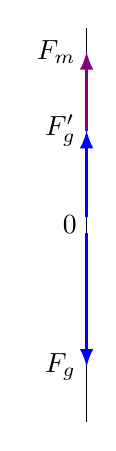
\begin{tikzpicture}

    \draw (0,-2.5) -- (0,2.5) 
    node [left,black] at(0,0) {$0$};

    \draw [blue,very thick,-latex] (0,-0.1) -- (0,-1.8) 
    node [left,black] {$F_g$};
    \draw [blue,very thick,-latex] (0,0.1) -- (0,1.2)
    node [left,black] {$F_g^\prime$};
    \draw [violet,very thick,-latex] (0,1.2) -- (0,2.2)
    node [left,black] {$F_m$};

  \end{tikzpicture}
\end{figure}
물체는 정지 상태에서 54 m 올라간 후 다시 정지하였으므로 승강기가 상승한 높이를 
$h$ 라 하면 승강기에 연결된 케이블이 승강기에 대해 해준 일은 다음과 같다.
\begin{align}
  W = \Delta U = mgh
\end{align}
승강기 대응추의 중력에 의한 힘을 $F_g^\prime$, 모터에 의한 힘을 $F_m$ 라 하자.
두 힘이 해준 일의 양은 승강기에 연결된 케이블이 해준 일의 양과 같다. 따라서,
\begin{align}
  W = (F_g^\prime+F_m)h = mgh  ,
\end{align}
이고 모터가 해준 일 $W_m$ 은 다음과 같다.
\begin{align}
  W_m = F_m\,h=(mg-F_g^\prime)h = (m-m^\prime)gh.
\end{align}
$m^\prime$ 은 승강기 대응추의 질량이다. 
3.0 분 동안 모터가 해준 평균 일률 $P_m$ 은 다음과 같다.
\begin{align}
  \begin{split}
    P_m &= \frac{W_m}{t} = \frac{(m-m^\prime)gh}{t}  \\
    &= \frac{(1\,200\,\mathrm{kg}-950\,\mathrm{kg})
    (9.8\,\mathrm{m/s^2})(54\,\mathrm{m})}{3.0\,\mathrm{\min}}
    =\frac{130\,000\,\mathrm{J}}{180\,\mathrm{s}} \\
    &= 7.4\times 10^2\,\mathrm{W}
  \end{split}
\end{align}
모터의 평균 일률은 $7.4\times 10^2\,\mathrm{W}$ 이다.

\vspace{1cm}

\noindent {\bf 문제 2 [20pt]}
그림~\ref{fig:2}과 같이 얼음덩어리가 경사각이 $\theta=50^\circ$이고
쓸림이 없는 경사면을 미끄러져 내려오고 있다. 이를 막기 위하여 크기가
50 N인 힘 $\vec{F}_r$로 얼음덩어리에 연결된 출을 잡아당기고
있다. 얼음덩어리가 경사면을 따라 거리 $d=0.50$ m만큼 미끄러져 내려왔을
때 운동에너지가 80 J 증가하였다. 만일 줄을 잡아당기지 않았다면
운동에너지는 얼마만큼 더 증가하겠는가?
\begin{figure}[ht]
  \centering
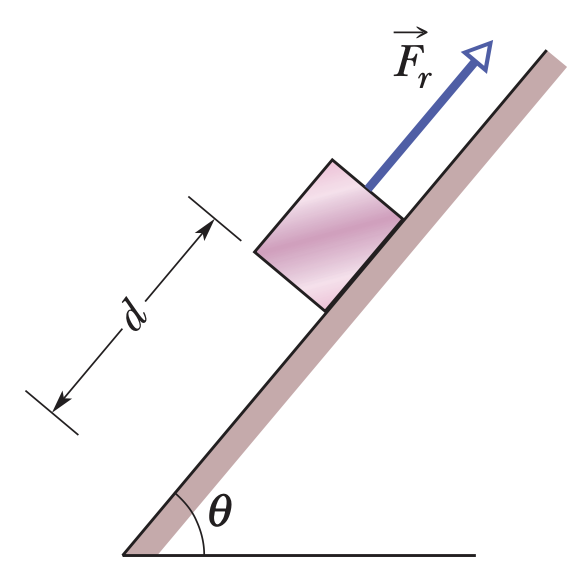
\includegraphics[scale=0.5]{Qfig8-2-20220328.png}
  \caption{문제 2}
  \label{fig:2}
\end{figure}

\noindent {\bf 풀이 : } 얼음덩어리의 자유 물체 다이어그램은 다음과 같다.
\begin{figure}[htbp]
  \centering
  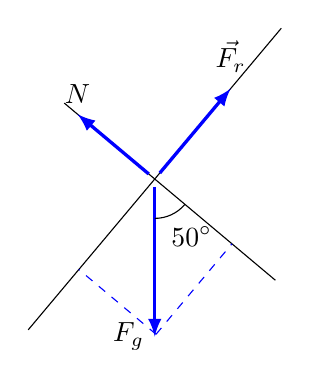
\begin{tikzpicture}
    \draw[rotate=50] (0,-2) -- (0,1.5); 
    \draw[rotate=50] (-2.5,0) -- (2.5,0);
    \draw[rotate=50] [blue,very thick,-latex] (0.1,0)--(1.5,0) 
            node [above=2,black] {$\vec{F_r}$};

    \draw[blue,very thick,-latex] (0,-0.1) -- (0,-2) 
    node [left,black] {$F_g$};
    \draw[rotate=50,blue,dashed] (-1.5,-1.28)--(-1.5,0); 
    \draw[rotate=50,blue,dashed] (-1.5,-1.28)--(0,-1.28); 
    \draw[rotate=50,blue,very thick,-latex] (0,0.1)--(0,1.28)
    node [above,black] {$N$};
    \draw[] (0,-0.5) arc(270:320:0.5) (0,0.5)
    node [below=35,right=2.5] {$50^\circ$};
  \end{tikzpicture}
\end{figure}

중력이 얼음덩어리에 해준 일을 $W_g$ 라 하자. 
힘 $\vec{F_r}$ 이 얼음덩어리에 해준 일 $W_r$ 이라 하면,
\begin{align}
  W_r = |\vec{F_r}| d \cos{180^\circ} = -|\vec{F_r}| d,
\end{align}
이고, 얼음덩어리의 운동에너지 변화량은 각 힘이 해준 일의 합이므로,
\begin{align}
  W_g+W_r = F_g d \cos{\phi} -|\vec{F_r}| d = 80\,\mathrm{J}.
\end{align}
따라서, 중력이 얼음덩어리에 해준 일은 다음과 같다.
\begin{align}
  \begin{split}
    W_g=80\,\mathrm{J}-W_r=80\,\mathrm{J}+|\vec{F_r}| d .
  \end{split}
\end{align}
$|\vec{F_r}|=50\,\mathrm{N}$, $d=0.50\,\mathrm{m}$ 이므로,
\begin{align}
  \begin{split}
    W_g&=80\,\mathrm{J}+|\vec{F_r}| d  \\
    &=80\,\mathrm{J}+(50\,\mathrm{N})(0.50\,\mathrm{m}) \\
    &=105\,\mathrm{J}
  \end{split}
\end{align}
힘 $\vec{F_r}$ 이 가해지지 않았더라면 중력이 해준 일이 모두 얼음덩어리의 운동 에너지를
변하게 하므로 그 때 운동 에너지는 $105\,\mathrm{J}$ 증가한다. 즉 줄을 잡아당겼을 때에 
비해 $25\,\mathrm{J}$ 만큼 더 증가한다.

\vspace{1cm}

\noindent {\bf 문제 3 [60pt]}
그림~\ref{fig:3}는 질량 $m=0.032$ kg인 작은 토막이 반지름 $R=12$ cm인
고리 모양의 쓸림이 없는 트랙 위를 미끄러지고 있다. 정지해 있던 토막을
바닥 위 높이 $h=5.0 R$인 점 $P$에서 놓았다. 
\begin{figure}[ht]
  \centering
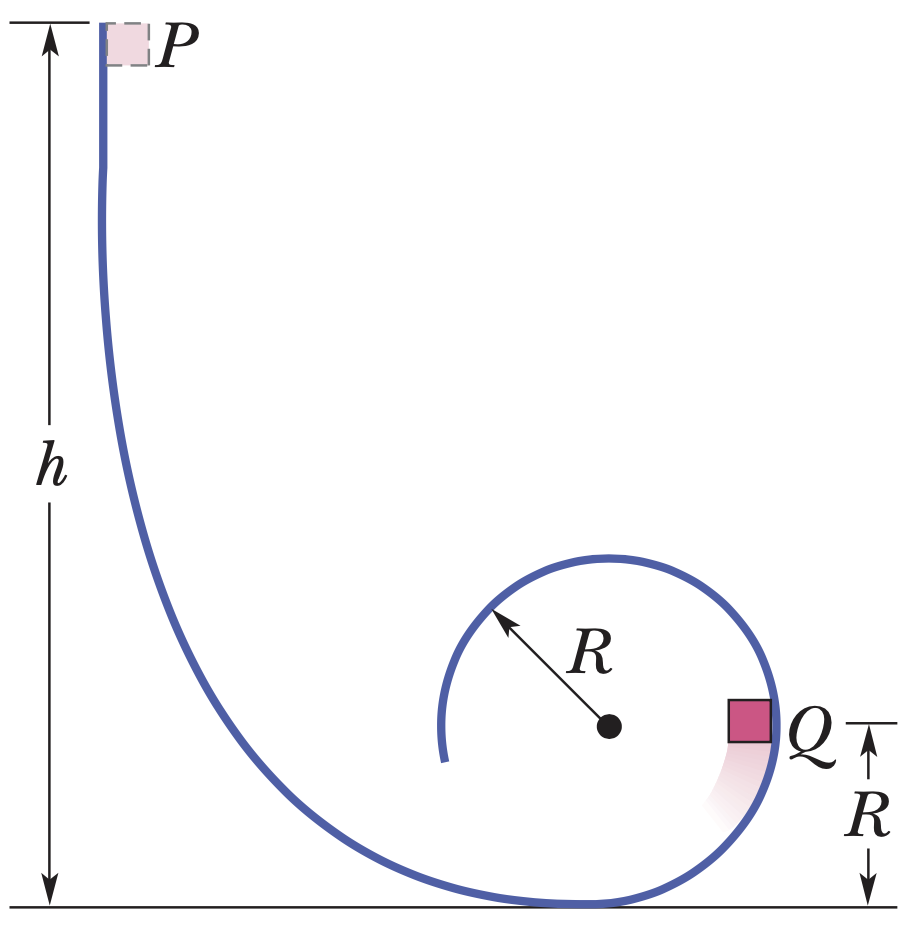
\includegraphics[scale=0.3]{Qfig8-3-20220328.png}
  \caption{문제 3}
  \label{fig:3}
\end{figure}

토막이 점 $P$에서
\begin{itemize}
\item[(가)] 점 $Q$
\item[(나)] 트랙의 꼭대기에 도달했을 때 중력이 토막에 한 일은 각각
  얼마인가?
\end{itemize}
트랙의 바닥에서 토막-지구 계의 중력 퍼텐셜 에너지를 $0$으로 하면 
\begin{itemize}
\item[(다)] 점 $P$
\item[(라)] 점 $Q$
\item[(마)] 트랙의 꼭대기에서의 중력 퍼텐셜에너지는 각각 얼마인가?
\item[(바)] 단순히 토막을 놓지 않고 일정 속력을 주어 토막을 아래로
  밀었다면 (가)에서 (마)까지의 답은 각각 증가, 감소, 불변 중 어느
  것인가? 
\end{itemize}
\noindent {\bf 풀이 : }
\begin{itemize}
  \item[(가)] 토막에 작용하는 힘은 중력 뿐이다. 따라서 중력이 해준 일과 
  토막의 운동에너지 변화량은 같다. 
  점 P와 점 Q 사이의 높이 차는 $h-R$ 이고 $h=5.0R$ 이므로
   중력 퍼텐셜 에너지의 차이는,
  \begin{align}
    mgh - mgR = 4mgR
  \end{align}
  이다. 역학적 에너지는 보존되므로 줄어든 중력 퍼텐셜 에너지 만큼 
  운동 에너지는 증가 하였다. 토막의 처음 운동에너지는 
  $0\,\mathrm{J}$ 이고 점 Q 에서의 운동 에너지를 $K_Q$ 라고 하자. 
  두 지점에서 운동 에너지 차이는,
  \begin{align}\label{eq:3-1}
    \begin{split}
      K_Q - 0\,\mathrm{J} &= mgh - mgR = 4mgR 
      =4(0.032\,\mathrm{kg})(9.80\,\mathrm{m/s^2})(0.12\,\mathrm{m})  \\
      &= 0.15\,\mathrm{J}
    \end{split}
  \end{align}
  운동 에너지 변화량은 $0.15\,\mathrm{J}$ 이므로 
  중력이 해준 일은 $0.15\,\mathrm{J}$ 이다.
  
  \item[(나)] 트랙의 꼭대기에 있을 때 점 $P$ 와의 중력 퍼텐셜 에너지 차이는,
  \begin{align}
    mgh - 2mgR = 3mgR
  \end{align}
  이다. 트랙의 꼭대기에서의 운동 에너지를 $K_t$ 라 하면 (\ref{eq:3-1}) 에 의해,
  \begin{align}
    \begin{split}
      K_t - 0\,\mathrm{J} &= mgh - 2mgR = 3mgR 
      =3(0.032\,\mathrm{kg})(9.80\,\mathrm{m/s^2})(0.12\,\mathrm{m})  \\
      &= 0.11\,\mathrm{J}
    \end{split}
  \end{align}
  운동 에너지 변화량은 $0.11\,\mathrm{J}$ 이므로 중력이 
  해준 일은 $0.11\,\mathrm{J}$ 이다.
  \item[(다)] 이제부터 토막이 바닥에 있을 때 중력 퍼텐셜 에너지를 0 J 이라 하자.
  바닥으로 부터 점 P 의 높이는 $h$ 이고 $h=5.0R$ 이므로
  점 P 에서의 중력 퍼텐셜 에너지를 $U_P$ 라고 하면,
  \begin{align}
    \begin{split}
      U_P &= mgh = 5mgR = 5(0.032\,\mathrm{kg})(9.80\,\mathrm{m/s^2})
      (0.12\,\mathrm{m})  \\
      &= 0.19\,\mathrm{J}
    \end{split}
  \end{align}
  점 P 에서의 중력 퍼텐셜 에너지는 $0.19\,\mathrm{J}$ 이다.
  \item[(라)] 바닥으로 부터 점 Q 의 높이는 $R$ 이므로 점 Q 에서의 중력 퍼텐셜 에너지를
  $U_Q$ 라 하면,
  \begin{align}
    \begin{split}
      U_Q &= mgR = (0.032\,\mathrm{kg})(9.80\,\mathrm{m/s^2})
      (0.12\,\mathrm{m})  \\
      &= 0.038\,\mathrm{J}
    \end{split}
  \end{align}
  점 Q 에서의 중력 퍼텐셜 에너지는 $0.038\,\mathrm{J}$ 이다.
  \item[(마)]
  바닥으로 부터 트랙의 꼭대기의 높이는 $2R$ 이므로 트랙의 꼭대기 
  에서의 중력 퍼텐셜 에너지를 $U_Q$ 라 하면,
  \begin{align}
    \begin{split}
      U_Q &= 2mgR = 2(0.032\,\mathrm{kg})(9.80\,\mathrm{m/s^2})
      (0.12\,\mathrm{m})  \\
      &=0.075\,\mathrm{J}
    \end{split}
  \end{align}
  트랙의 꼭대기 에서의 중력 퍼텐셜 에너지는 $0.075\,\mathrm{J}$ 이다.
  \item[(바)]
  일정 속력을 주어 토막을 아래로 밀었을 때 점 P 에서의 운동에너지를 $K_P$ 이라 하자.
  임의의 지점 X 에서의 운동 에너지를 $K_X$, 중력 퍼텐셜 에너지를 $U_X$ 라
  하면 역학적 에너지 보존에 의해,
  \begin{align}
    K_P+mgh = K_X+U_X
  \end{align}
  이다. 토막이 지점 X 까지 움직이는 동안 중력이 토막에 해준 일을 $W_X$ 라 하면 
  중력이 해준 일은 토막의 운동에너지 변화량과 같으므로,
  \begin{align}
    W_X = K_X-K_P=mgh-U_X,
  \end{align}
  이다. 따라서 $K_P$ 에 의존하지 않는다. 또한, 
  지점 X 에서의 중력 퍼텐셜 에너지 $U_X$ 는 바닥으로 부터의 높이와 토막의 질량에만 
  의존하므로 (가), (나)의 답은 불변이고 (다), (라), (마) 의 답 또한 불변이다.
\end{itemize}

\end{document}